%%%%%%%%%%%%%%%%%%%%%%%%%%%%%% DISCLAIMER %%%%%%%%%%%%%%%%%%%%%%%%%%%%%%
% The author of the thesis remains responsible for fulfilling all
% requirements.
%%%%%%%%%%%%%%%%%%%%%%%%%%%%%%%%%%%%%%%%%%%%%%%%%%%%%%%%%%%%%%%%%%%%%%%%

\RequirePackage{lineno}
\documentclass[12pt,reqno,french]{DMSE-Thesis}

%%%%%%%%%%%%%%%%%%%%%%%%%%%%%%%%%%%%%%%%%%%%%%%%%%%%%%%%%%%%%%%%%%%%%%%%
% Typing Aids
%----------------------------------------------------------------------%
\newcommand{\dmse}{Department of Materials Science and Engineering}
% Your macros can be loaded here:
% \usepackage{My-Typing-Aids}

%%%%%%%%%%%%%%%%%%%%%%%%%%%%%%%%%%%%%%%%%%%%%%%%%%%%%%%%%%%%%%%%%%%%%%%%
% REQUIRED USER INPUT
%----------------------------------------------------------------------%
% Author and title.
\author{Ian Wise}
\title{Mini-Thesis}

% Pursued Degree.
% Default: Doctor of Philosophy.
\degree{Bachelor of Science in Engineering}  

\advisor{Professor Frank Ernst}

\department{\dmse}     

% Graduation month.
\graduationmonth{May}      

% Graduation year.
\graduationyear{2021}

% Set line spacing. Use \onehalfspacing, \doublespacing, or \protect\setstretch{real number}.
\doublespacing

%%%%%%%%%%%%%%%%%%%%%%%%%%%%%%%%%%%%%%%%%%%%%%%%%%%%%%%%%%%%%%%%%%%%%%%%
% ESSENTIAL PACKAGES 
% ----------------------------------------------------------------------%
% Graphics, figures.
\usepackage[pdftex]{graphicx}

% The following makes graphicx work with pdf and jpg files. Files with
% same names and different extensions will be recognized in sequential
% order. Note that pdflatex is quicker with pdf files.
\DeclareGraphicsExtensions{.pdf, .jpg}

% Generate bibliography and citations with natbib package.
\RequirePackage[comma, super, numbers, sort&compress]{natbib}


% Enable hyperlinks.
\usepackage{hyperref} 

%%%%%%%%%%%%%%%%%%%%%%%%%%%%%%%%%%%%%%%%%%%%%%%%%%%%%%%%%%%%%%%%%%%%%%%%
% OPTIONAL PACKAGES
%----------------------------------------------------------------------%
% The following packages may be useful. However, to minimize compilation
% time, you should only activate them when needed.

% Upright Greek letters.
% Normally, you typeset Greek letters in math mode. They will then be typeset in italics, appropriate for variables. However, there are many instances in which Greek letters are not used for variables. For instance, the Greek letters used for indicating thermodynamic phases (e.g. alpha-Sn) or spectral lines (e.g. Cu-K_alpha). The following package provides support for upright Greek letters.
\usepackage{FE-uGreek}

% Subfigures of figures.
%\usepackage{subcaption}

% Landscape environment.
%\usepackage{pdflscape} 

% Tables spanning more than one page.
%\usepackage{longtable}

% PDFPages imports entire PDF pages.
% \usepackage[final]{pdfpages}

% For comment environment.
% \usepackage{verbatim} 

% Wrapfig wraps text around tables and figures.
% \usepackage{wrapfig}

% Tables with cells spanning multiple rows.
% \usepackage{multirow}

% Tables with captions and notes.
% \usepackage{threeparttable}

% Better Footnotes.
% \usepackage{footnote}

% Makes tables handle footnotes correctly.
% \makesavenoteenv{tabular}

%%%%%%%%%%%%%%%%%%%%%%%%%%%%%%%%%%%%%%%%%%%%%%%%%%%%%%%%%%%%%%%%%%%%%%%%
% Font Settings
%----------------------------------------------------------------------%
% The style file "DMSE-Thesis.sty" provides detailed settings for fonts
% and text appearance. This loads the style file:

\usepackage{DMSE-Thesis}


%%%%%%%%%%%%%%%%%%%%%%%%%%%%%%%%%%%%%%%%%%%%%%%%%%%%%%%%%%%%%%%%%%%%%%%%
\begin{document}
%%%%%%%%%%%%%%%%%%%%%%%%%%%%%%%%%%%%%%%%%%%%%%%%%%%%%%%%%%%%%%%%%%%%%%%%

\frontmatter
%\pagenumbering{roman}

% Title page.
\maketitle

% Page for signatures of committee members.
% For the final turn in, you do not need this page signed, just dated.
% to date this page, cludgy way to do it is replace Signature/Date with the Date
% Found in the CWRU-thesis.cls file, line 327
\signaturepage
\sign[Advisor]{Advisor Name}{Chair}{\dmse}
\sign{Committee Member Name}{Member}{\dmse}
\sign{Committee Member Name}{Member}{\dmse}
\sign{Committee Member Name}{Member}{Department}

% Title and signature page have fixed linespacing. For the following,
% set the linespacing here.
\onehalfspacing
% \doublespacing
% \protect\setstretch{real number}

% Copyright page (optional). You do not need a copyright page unless you
% are actually applying for a copyright.
% \copyrightpage

% Dedication page (optional). Indicate linebreaks by "\\".
\dedication{Dedicated to Progress in\\
  Materials Science and Engineering}

% Preface (optional).
% \preface
% \input 00-Preface.tex

% Table of Contents will be automatically generated and placed here.
\tableofcontents

% Add line numbers.
\linenumbers

% List of Tables and List of Figures will be automatically generated
% and placed here.
\listoftables	
\listoffigures		

% Acknowledgements (optional).
\acknowledgements
\noindent
Your acknowledgements here: Advisor, committee, colleagues, engineers, staff, funding agencies, etc.

%%% Local Variables:
%%% mode: latex
%%% TeX-master: "DMSE-Thesis"
%%% End:


% Abstracts must not exceed 350 words in dissertations and 150
% words in other theses.
\abstract
Your abstract here. Check limits for number of words. Usually, abstracts must not exceed 350 words in dissertations and 150 words in other theses. The abstract should not replace the introduction. It should include the most important results \emph{and} the most important conclusions~-- how this work has advanced the field.

%%% Local Variables:
%%% mode: latex
%%% TeX-master: "DMSE-Thesis"
%%% End:
 

\mainmatter             
\pagenumbering{arabic} 

% Up to this point, the hyperlink color was black (default) to avoid
% that tables of contents, figures, etc in the front matter entirely
% appear in color. Here, change the hyperlink and citation color to a
% blue hue that is clearly distinct from black (also when printed in
% black and white), but not disturbing in long lists of references.
\definecolor{linkcol}{rgb}{0.,0.,0.5}
\definecolor{citecol}{rgb}{0.,0.,0.5}
%\definecolor{headcol}{rgb}{0.4,0.4,0.4}

\chapter{Introduction}

\section{Testing Citations and Bibliography}
\label{sec:testbib}

Here is a nice paper.\cite{ernst-2017-142} 


\section{Testing Figures}
\label{sec:testfig}

Here is a nice figure.

\begin{figure}[t]
  \centering

  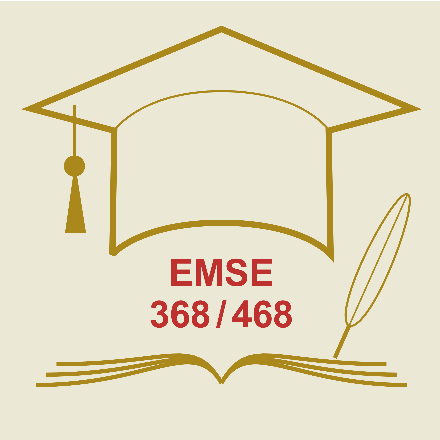
\includegraphics[width=0.4\hsize]{I:/Documents/1CWRU/Semester_3.99/EMSE_368/version_control/FIG/Logo-368-468.pdf}
  \caption{Logo of EMSE-368/468.}
  \label{fig:logo}
\end{figure}

We can refer to it as \ref{fig:logo}.


% Uncomment for bibliography on each chapter.
% \bibliographystyle{plainnat}				
% \markright{\textit{Bibliography}}
% \renewcommand{\chaptername}{}
% \bibliography{my_references}

% \vfill


%%% Local Variables:
%%% mode: latex
%%% TeX-master: "DMSE-Thesis"
%%% End:

\chapter{Literature Review} 
\label{ch:lit}


% Uncomment for bibliography on each chapter.
% \bibliographystyle{plainnat}				
% \markright{\textit{Bibliography}}
% \renewcommand{\chaptername}{}
% \bibliography{my_references}

% \vfill

%%% Local Variables:
%%% mode: latex
%%% TeX-master: "DMSE-Thesis"
%%% End:

\chapter{Methods}

\section{Experimental Methods}
\label{sec:expmeth}

\section{Computational Methods}
\label{sec:compmeth}


% Uncomment for bibliography on each chapter.
% \bibliographystyle{plainnat}				
% \markright{\textit{Bibliography}}
% \renewcommand{\chaptername}{}
% \bibliography{my_references}

% \vfill


%%% Local Variables:
%%% mode: latex
%%% TeX-master: "DMSE-Thesis"
%%% End:

\chapter{Results}

\section{Experimental Results}


% Uncomment for bibliography on each chapter.
% \bibliographystyle{plainnat}				
% \markright{\textit{Bibliography}}
% \renewcommand{\chaptername}{}
% \bibliography{my_references}

% \vfill


%%% Local Variables:
%%% mode: latex
%%% TeX-master: "DMSE-Thesis"
%%% End:

\chapter{Discussion}


% Uncomment for bibliography on each chapter.
% \bibliographystyle{plainnat}				
% \markright{\textit{Bibliography}}
% \renewcommand{\chaptername}{}
% \bibliography{my_references}

% \vfill


%%% Local Variables:
%%% mode: latex
%%% TeX-master: "DMSE-Thesis"
%%% End:

\chapter{Conclusions}


% Uncomment for bibliography on each chapter.
% \bibliographystyle{plainnat}				
% \markright{\textit{Bibliography}}
% \renewcommand{\chaptername}{}
% \bibliography{my_references}

% \vfill

%%% Local Variables:
%%% mode: latex
%%% TeX-master: "DMSE-Thesis"
%%% End:

\include{07-Futurework}
% \include{08-Summary}
\bibliography{../BIB/DMSE-Thesis.bib}

% \vfill


%%% Local Variables:
%%% mode: latex
%%% TeX-master: "DMSE-Thesis"
%%% End:

\appendix
\include{app_pprofile} % HHP profile
\include{app_specimens} % master list
\include{app_thesis_prep} % programs used to generate this document
\include{app_figs} % list of microscope figures used in text


% 

% You can choose between:

% (a) One bibliography at the end of the document. This is appropriate
% for numbered citations (default).
\bibliographystyle{plainnat}	

% You can choose the title of the bibliography here:
% \renewcommand{\bibname}{My Own Title for References}


% (b) One bibliography at the end of the document plus a bibliography
% for each chapter. This only makes sense for "naming" bibliography
% styles, not for "numbering" styles: A style with numbering will give
% separate and unrelated numbers in each bibliography.

% This chooses an unnumbered bibliography style. 
% \bibliographystyle{unsrt} 

% You can choose the title of the global bibliography here:
% \renewcommand{\bibname}{Complete References}

% Include/uncomment the following lines at the end of each chapter .tex file:
% \bibliographystyle{plainnat}				
% \markright{\textit{Bibliography}}
% \renewcommand{\chaptername}{}
% \bibliography{my_references}

% To generate all bibliographies, proceed as follows:
% (1) Activate package chapterbib with option rootbib.
% \usepackage[rootbib]{chapterbib}
% (2) Run LaTeX.
% (3) Run BibTeX on the root file.
% (4) Deactivate option rootbib (i.e. load package without that option).
% \usepackage{chapterbib}
% (5) Run LaTeX.
% (6) Run BibTeX on each included file.
% (7) Run LaTeX twice.


\end{document}
\end


%%% Local Variables: 
%%% mode: tex-pdf
%%% TeX-master: t
%%% End: 


				


